\documentclass[border=8pt]{standalone}
\usepackage[utf8]{inputenc}
\usepackage[T1]{fontenc}
\usepackage[scaled]{helvet}
\renewcommand{\familydefault}{\sfdefault}
\usepackage{tikz}
\usetikzlibrary{positioning,arrows.meta,fit,backgrounds,shapes.geometric}
\tikzset{
  uc/.style={ellipse, draw, thick, fill=white, font=\scriptsize, align=center, minimum width=5.2cm, minimum height=0.62cm, inner sep=0.5pt, text width=4.2cm},
  pkg/.style={draw, thick, rounded corners=2pt, inner sep=6pt},
  ptitle/.style={font=\footnotesize\bfseries, anchor=north west},
  link/.style={thick},
  gen/.style={thick, -{Triangle[open, length=3mm, width=3mm]}}
}
\newcommand{\actor}[3]{% name, position, label
  \begin{scope}[shift={#2}]
    \draw[thick] (0,0.55) circle (0.22);
    \draw[thick] (0,0.33) -- (0,-0.25);
    \draw[thick] (-0.35,0.15) -- (0.35,0.15);
    \draw[thick] (0,-0.25) -- (-0.28,-0.7);
    \draw[thick] (0,-0.25) -- (0.28,-0.7);
    \node[font=\footnotesize, align=center, anchor=north] at (0,-0.75) {#3};
    \coordinate (#1) at (0,0);
  \end{scope}}
% \pk{id}{x}{y}{titulo}{lista de (nombre,etiqueta)}
\newcommand{\ucs}[4]{% id, x, y, list
  \foreach \lab [count=\i] in {#4} {
    \node[uc] (#1-\i) at (#2, #3-0.78*\i) {\lab};
  }}
\begin{document}
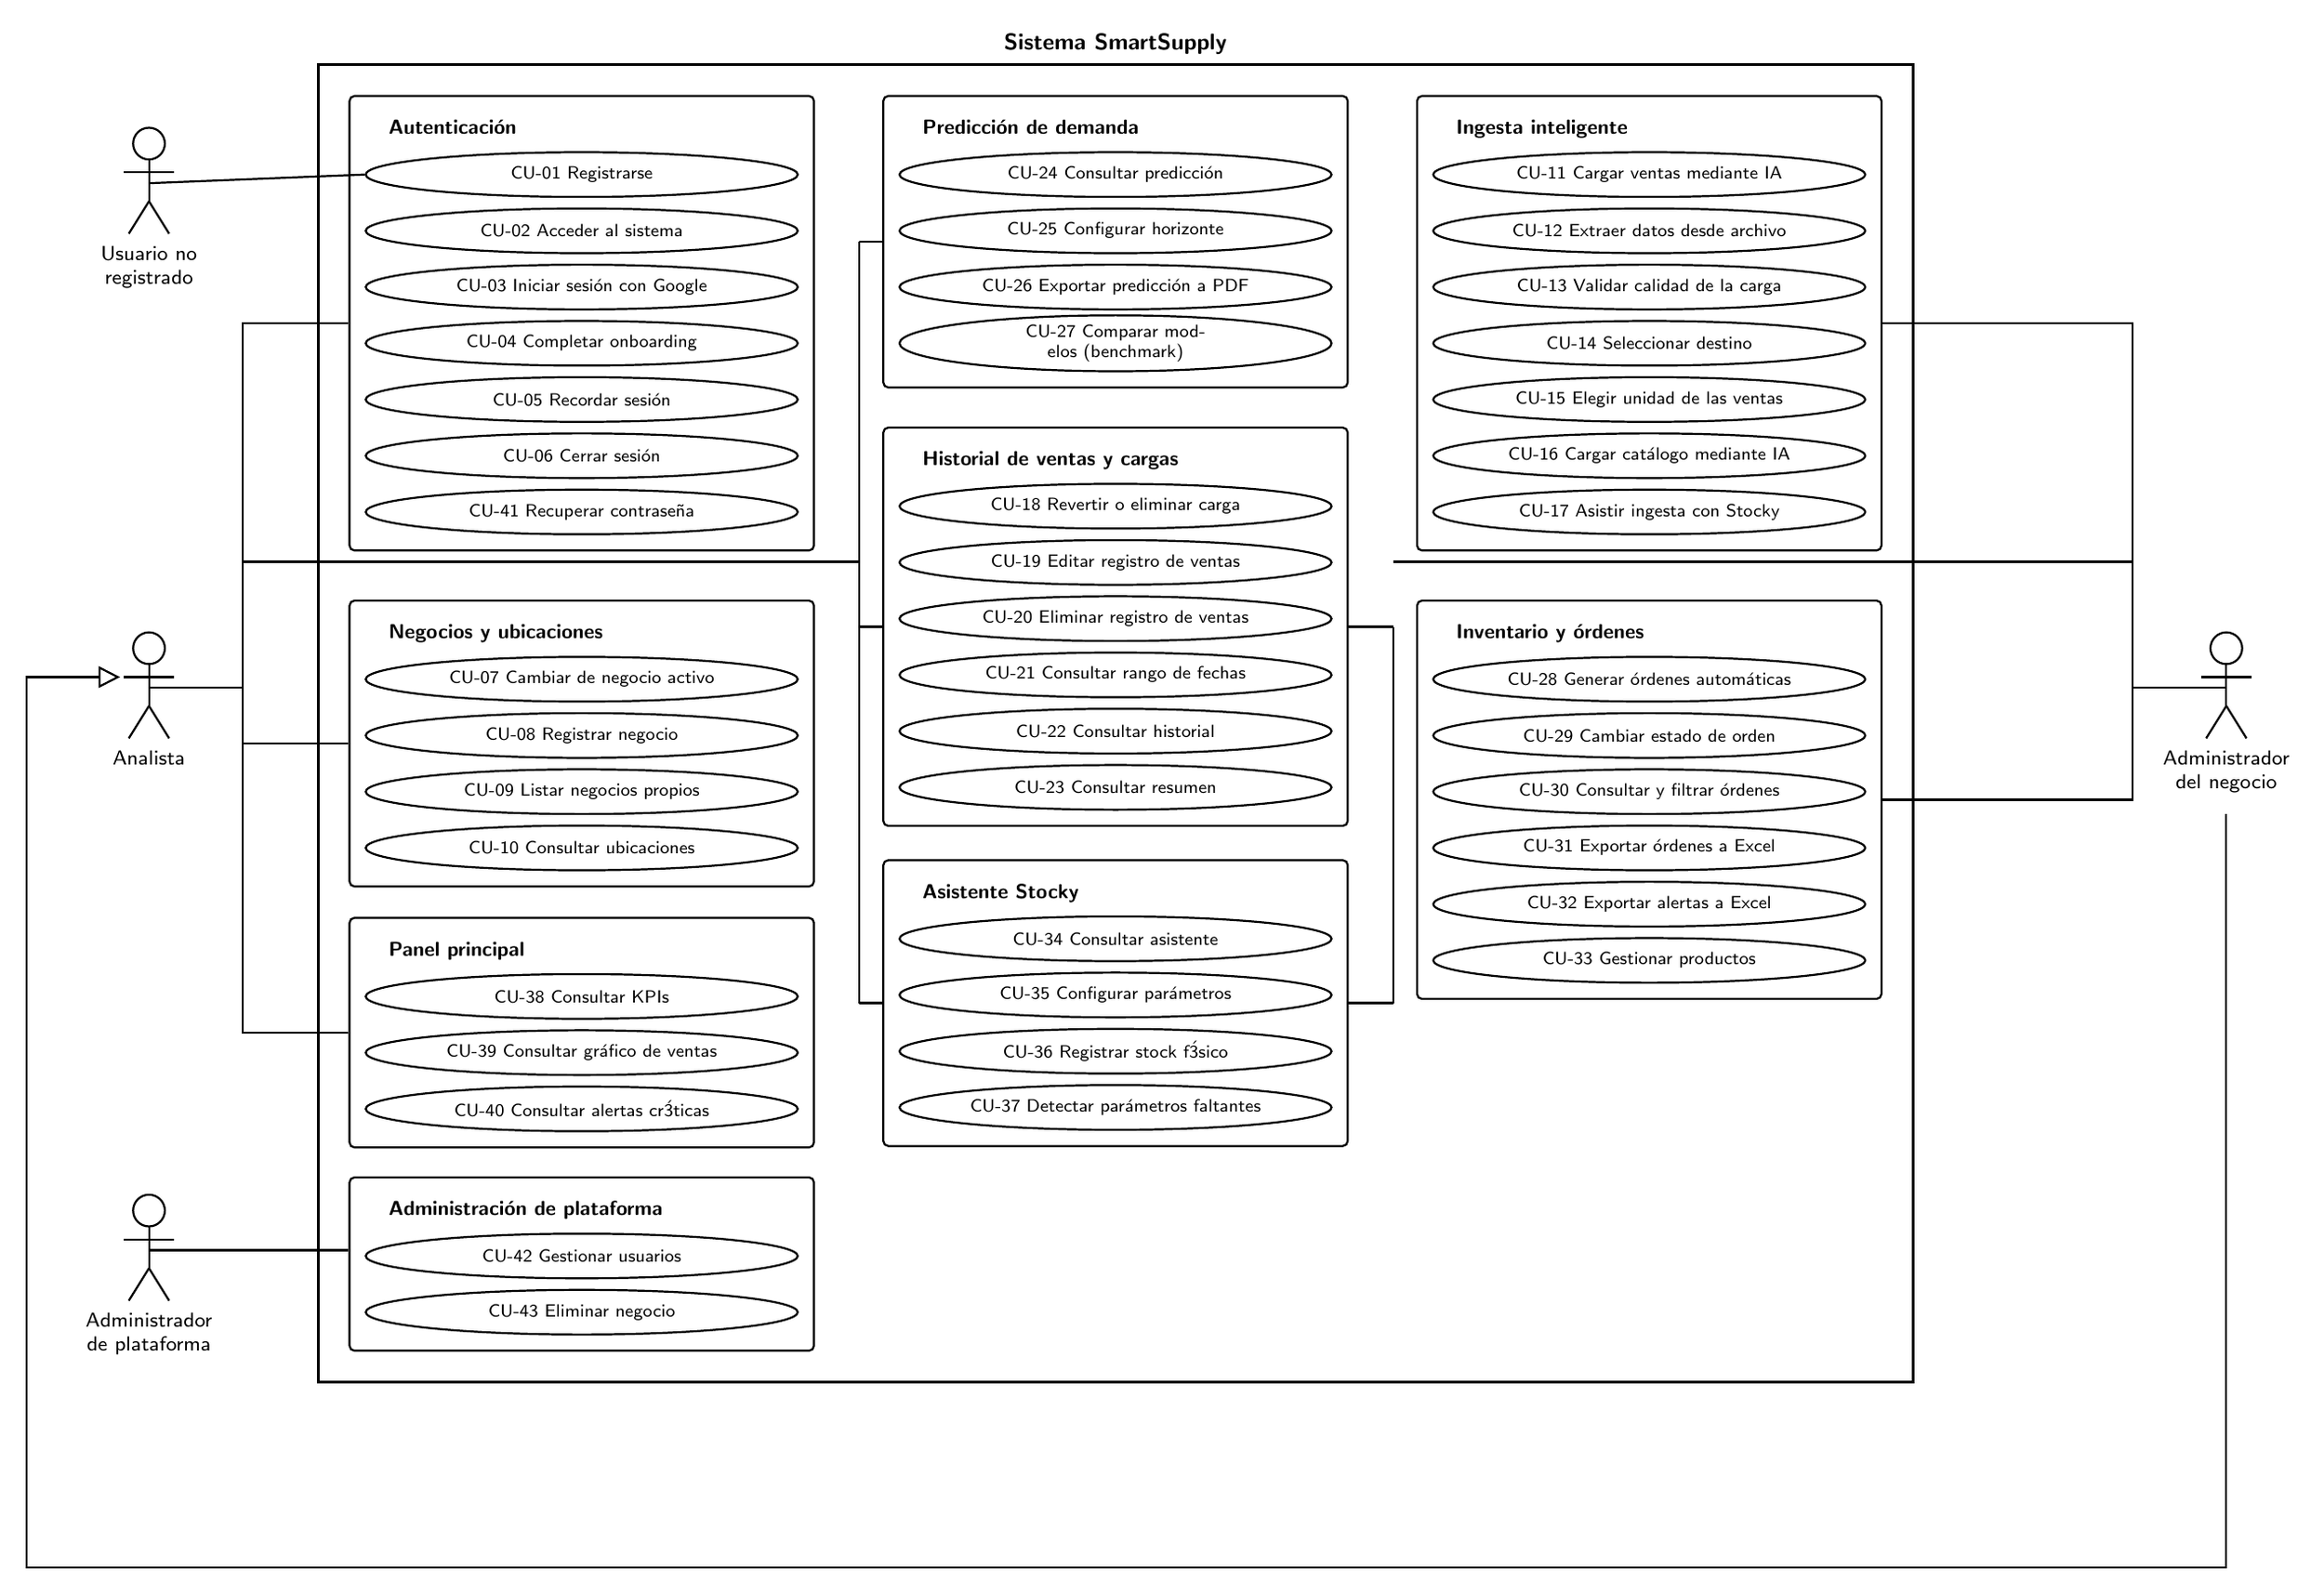
\begin{tikzpicture}
% Columna 1 (x=0)
\node[ptitle] (t1) at (0,0) {Autenticación};
\ucs{a}{2.8}{-0.1}{{CU-01 Registrarse},{CU-02 Acceder al sistema},{CU-03 Iniciar sesión con Google},{CU-04 Completar onboarding},{CU-05 Recordar sesión},{CU-06 Cerrar sesión},{CU-41 Recuperar contraseña}}
\node[ptitle] (t2) at (0,-7.0) {Negocios y ubicaciones};
\ucs{b}{2.8}{-7.1}{{CU-07 Cambiar de negocio activo},{CU-08 Registrar negocio},{CU-09 Listar negocios propios},{CU-10 Consultar ubicaciones}}
\node[ptitle] (t3) at (0,-11.4) {Panel principal};
\ucs{c}{2.8}{-11.5}{{CU-38 Consultar KPIs},{CU-39 Consultar gráfico de ventas},{CU-40 Consultar alertas críticas}}
\node[ptitle] (t4) at (0,-15.0) {Administración de plataforma};
\ucs{k}{2.8}{-15.1}{{CU-42 Gestionar usuarios},{CU-43 Eliminar negocio}}
% Columna 2 (x=7.4)
\node[ptitle] (t5) at (7.4,0) {Predicción de demanda};
\ucs{f}{10.2}{-0.1}{{CU-24 Consultar predicción},{CU-25 Configurar horizonte},{CU-26 Exportar predicción a PDF},{CU-27 Comparar modelos (benchmark)}}
\node[ptitle] (t6) at (7.4,-4.6) {Historial de ventas y cargas};
\ucs{e}{10.2}{-4.7}{{CU-18 Revertir o eliminar carga},{CU-19 Editar registro de ventas},{CU-20 Eliminar registro de ventas},{CU-21 Consultar rango de fechas},{CU-22 Consultar historial},{CU-23 Consultar resumen}}
\node[ptitle] (t7) at (7.4,-10.6) {Asistente Stocky};
\ucs{h}{10.2}{-10.7}{{CU-34 Consultar asistente},{CU-35 Configurar parámetros},{CU-36 Registrar stock físico},{CU-37 Detectar parámetros faltantes}}
% Columna 3 (x=14.8)
\node[ptitle] (t8) at (14.8,0) {Ingesta inteligente};
\ucs{d}{17.6}{-0.1}{{CU-11 Cargar ventas mediante IA},{CU-12 Extraer datos desde archivo},{CU-13 Validar calidad de la carga},{CU-14 Seleccionar destino},{CU-15 Elegir unidad de las ventas},{CU-16 Cargar catálogo mediante IA},{CU-17 Asistir ingesta con Stocky}}
\node[ptitle] (t9) at (14.8,-7.0) {Inventario y órdenes};
\ucs{g}{17.6}{-7.1}{{CU-28 Generar órdenes automáticas},{CU-29 Cambiar estado de orden},{CU-30 Consultar y filtrar órdenes},{CU-31 Exportar órdenes a Excel},{CU-32 Exportar alertas a Excel},{CU-33 Gestionar productos}}
% Paquetes
\begin{scope}[on background layer]
\node[pkg, fit=(t1)(a-1)(a-7)] (P1) {};
\node[pkg, fit=(t2)(b-1)(b-4)] (P2) {};
\node[pkg, fit=(t3)(c-1)(c-3)] (P3) {};
\node[pkg, fit=(t4)(k-1)(k-2)] (P4) {};
\node[pkg, fit=(t5)(f-1)(f-4)] (P5) {};
\node[pkg, fit=(t6)(e-1)(e-6)] (P6) {};
\node[pkg, fit=(t7)(h-1)(h-4)] (P7) {};
\node[pkg, fit=(t8)(d-1)(d-7)] (P8) {};
\node[pkg, fit=(t9)(g-1)(g-6)] (P9) {};
\node[draw, very thick, inner sep=12pt, fit=(P1)(P4)(P8)(P9)] (S) {};
\end{scope}
\node[font=\small\bfseries, anchor=south] at (S.north) {Sistema SmartSupply};
% Actores
\actor{nr}{(-3.2,-1.0)}{Usuario no\\registrado}
\actor{an}{(-3.2,-8.0)}{Analista}
\actor{pa}{(-3.2,-15.8)}{Administrador\\de plataforma}
\actor{adm}{(25.6,-8.0)}{Administrador\\del negocio}
% Pasillos
\coordinate (gy1) at (0,{(-6.25)});        % entre Autenticación y Negocios
\coordinate (cx12) at ({6.65},0);          % entre columnas 1 y 2
\coordinate (cx23) at ({14.05},0);         % entre columnas 2 y 3
% Asociaciones del Analista
\draw[link] (nr) -- (a-1.west);
\draw[link] (an) -- ++(1.3,0) coordinate (bus);
\draw[link] (bus) |- (P1.west);
\draw[link] (bus) |- (P2.west);
\draw[link] (bus) |- (P3.west);
\draw[link] (bus |- gy1) -- (cx12 |- gy1);
\draw[link] (cx12 |- P5.west) -- (cx12 |- P7.west);
\draw[link] (cx12 |- P5.west) -- (P5.west);
\draw[link] (cx12 |- P6.west) -- (P6.west);
\draw[link] (cx12 |- P7.west) -- (P7.west);
\draw[link] (pa) -- (P4.west |- pa);
% Asociaciones del Administrador del negocio
\draw[link] (adm) -- ++(-1.3,0) coordinate (bus2);
\draw[link] (bus2) |- (P8.east);
\draw[link] (bus2) |- (P9.east);
\draw[link] (bus2 |- gy1) -- (cx23 |- gy1);
\draw[link] (cx23 |- P6.east) -- (cx23 |- P7.east);
\draw[link] (cx23 |- P6.east) -- (P6.east);
\draw[link] (cx23 |- P7.east) -- (P7.east);
% Generalización: Administrador del negocio hereda de Analista
\draw[gen] ([yshift=-1.75cm]adm) -- ([yshift=-1.75cm]adm |- S.south) -- ++(0,-0.8) -| (-4.9,-7.85) -- (-3.6,-7.85);
\end{tikzpicture}
\end{document}
